\begin{comment}
\end{comment}

\chapter{Étude des codes polaires convolutifs}

Le problème de communication classique est défini comme suit.
Deux acteurs, 
qui se nomment Arthur et Béatrice pour faire changement\footnote{
  Une recherche en ligne vous démontrera que beaucoup d'attention a été donnée 
  à Alice et Bob. 
},
veulent échanger de l'information.
Dans ce cas,
supposons qu'Arthur cherchent à envoyer un message à Béatrice qui se trouve
des kilomètres plus loin.
Pour ce faire,
Arthur utilise son téléphone cellulaire et envoie un texto à Béatrice.
Une fois le message composé,
celui-ci est converti en une séquence de nombres binaires (des 0 et des 1)
qui sera transmise via des ondes radios jusqu'au téléphone de Béatrice
qui devra reconvertir la séquence de 0 et de 1 en message intelligible.

Cependant, 
l'histoire ne s'arrête pas là,
puisque lors de la transmission du signal dans l'atmosphère,
il est fort probable que celui-ci soit corrompu en 
raison d'une interaction indésirée.
En autre, 
cela peut être causé par la présence d'autres ondes ou d'un obstacle 
sur le trajet du signal.
La solution à ce problème est alors de transmettre une séquence de nombres binaires
plus longue que ce qui est nécessaire en espérant que l'information supplémentaire
nous aide à retrouver le message initial malgré la présence d'erreurs.

Dans ce chapitre,
je vais d'abord reformuler ce problème dans un langage mathématique plus formel.  
Par la suite, 
je vais présenter les réseaux de tenseurs,
un outil mathématique qui va m'être très utile pour décrire les codes polaires 
ainsi qu'une généralisation de ces derniers, les codes polaires convolutifs.
Ces codes sont très importants puisque les codes polaires sont au coeur 
de la technologie de communication 5G~\cite{bioglio_design_2021} et que toutes améliorations de ceux-ci
a un grand potentiel d'application.
À cet effet, le chapitre se termine par une présentation d'un article scientifique
dans lequel j'identifie les régimes où les performances des codes polaires convolutifs sont 
les plus impressionnantes.

\section{Communication classique et correction d'erreurs}

L'unité fondamentale de l'information est le bit.
Un bit prend la valeur 0 ou 1 et correspond à la quantité 
d'information acquiérie après avoir appris la réponse 
à une question ayant deux choix de réponses (oui et non par exemple).
Formellement, un bit est un élément du corps fini de cardinalité 2 noté $\bit = \qty{0, 1}$.
La multiplication dans $\bit$ est définie comme à l'habitude
et l'addition est définie modulo 2, soit que $1 + 1 = 0$.

Je m'intéresse au cas où Arthur veut transmettre une séquence 
de $k$ bits $\vb{x} \in \bit^k$ en utilisant un canal bruité $\canal$.
Dans cette thèse,
je vais me limiter à une définiton simple d'un canal bruité,
bien qu'il soit possible de généraliser cette notion. 
Le canal bruité que je considère est le canal binaire symétrique.
Celui-ci est une fonction probabiliste $\mathcal \canal_p: \bit \to \bit$
qui, après avoir reçu le bit $b$ comme entrée, 
retourne le même bit $b$ avec probabilité $1 - p$ et retourne le
bit opposé $1 + b$ avec probabilité $p$.
Il est commun de nommer $p$ la probabilité de renversement 
ou la probabilité d'erreur.

Dans le cas où $k > 1$ bits sont transmis via un canal bruité $\canal_p$,
un canal effectif $\canal_p^k$ composé de $k$ copies de $\canal_p$
est considéré.
Par exemple,
si le message $00000$ est transmis,
le message $01010$ est reçu avec probabilité $p^2(1 - p)^3$ 
tandis que le message $11111$ est reçu avec probabilité $p^5$.
De façon générale, 
la probabilité que le message original soit reçu sans erreur est de $(1 - p)^k$.
Cette probabilité décroit exponentiellement avec la taille du message 
et il est rapidement improbable que cela se produise.

Pour contrer ce problème,
chaque message original $\vb x \in \bit^k$ est encodé dans une autre séquence 
unique de bits $\vb{y} \in \bit^n$ telle que $n > k$.
Comme le nombre de messages dans $\bit^k$ est inférieur au nombre
de séquences dans $\bit^n$,
seul un sous-espace $\code \subset \bit^n$ est utilisé.
Ce sous-espace $C$ définit un code correcteur d'erreurs
de $k$ bits logiques et de $n$ bits physiques 
et un élément de $C$ est nommé mot-code.

\begin{table}[t]
  \caption{Exemple d'encodage de 2 bits vers 6 bits}
  \label{tab:exemple_encodage}
  \begin{center}
    \begin{tabular}[c]{cc}
      \textbf{Message} & \textbf{Mot-code} \\
      \hline
      00 & 000000 \\
      01 & 101010 \\
      10 & 010101 \\
      11 & 111111
    \end{tabular}
  \end{center}
\end{table}

Le tableau~\ref{tab:exemple_encodage} illustre un exemple de code correcteur
encodant 2 bits logiques à l'aide de 6 bits physiques.
En utilisant ce code correcteur,
Béatrice est en mesure de retrouver le message initial qu'Arthur lui a
envoyé s'il y a au plus une erreur qui affecte les 6 bits transmis. 
Par exemple, si le message 01 est transmis à l'aide du mot-code 
101010 et que la séquence 111010 est reçue, 
il est aisé, en comparant cette séquence avec les différents 
mots-codes, d'identifier le message envoyé. 
Par contre, 
si deux erreurs affectait le mot-code générant la séquence 111110, 
Béatrice concluerait à tord que le message 11 a été envoyé par Arthur.
L'opération qui consiste à essayer de retrouver le message original à partir
de la séquence reçue se nomme décodage 
et une erreur logique est une erreur à la suite du décodage.

Pour cet exemple,
la probabilité de transmettre un message de 2 bits sans encodage avec succès 
est de $(1 - p)^2$. 
En comparaison,
lorsque l'encodage de 6 bits est utilisé, 
la probabilité que Béatrice soit en mesure de retrouver le message original 
sans erreur logique est de $(1 - p)^6 + 6p(1 - p)^5$.
Ainsi, si $p \lesssim 0.22$, il est avantageux d'utiliser le code correcteur.

\subsection{Capacité des canaux bruités}

Le défi de la correction d'erreur est de construire des codes correcteurs 
qui réduisent considérablement la probabilité d'une erreur logique sans utiliser 
un trop grand nombre de bits supplémentaires.
À cet effet, c'est en 1948 que Claude Shannon a démontré la plus grande valeur 
de rendement $R = k/n$ qui peut être transmise 
via un canal bruité~\cite{shannon_mathematical_1948}.
Plus précisement,
la capacité $\capacite$ d'un canal bruité est le rendement maximum 
que peuvent transmettre plusieurs copies du canal tel que la probabilité d'une 
erreur logique tend vers 0 lorsque $n \to \infty$.
Autrement dit,
pour un canal de capacité $\capacite$, 
il existe une famille de codes $\qty{C_i}_{i\in\mathbb N}$ avec 
$k_i / n_i \to \capacite$ telle que la probabilité d'une erreur de 
décodage décroit exponentiellement avec $i$.

La capacité d'un canal est calculé à partir de l'information mutuelle~\footnote{
  Les concepts importants de la théorie de l'information, dont l'entropie
  et l'information mutuelle sont présentés à l'annexe~\ref{chap:theo_info}.
} 
selon
\begin{equation}
  \capacite = \max_{\Pr_X(x)} I(X ; Y),
\end{equation}
avec $X$ la variable aléatoire transmise et $Y$ la variable aléatoire reçue.
Dans ce cas,
l'information mutuelle $I(X ; Y)$ est interprété comme la fraction maximale
de bits non erronés qui peuvent être reçus par bit envoyé.
Cette quantité dépend généralement de la probabilité d'envoyer chaque bit
et il est alors optimal de choisir la probabilité qui maximise l'information mutuelle.
Lors de l'introduction aux codes polaires à la fin de ce chapitre,
j'utiliserai l'information mutuelle pour comparer la performance de divers canaux.

Pour le canal binaire symétrique $\canal_p$, 
il est prouvé~\cite{shannon_mathematical_1948} que l'information mutuelle
est maximisée par une probabilité uniforme sur $X$. 
La capacité est alors
\begin{equation}
  \capacite(\canal_p) = 1 - H_2(p)
\end{equation}
avec l'entropie binaire $H_2(p) = -p \log(p) - (1 - p)\log(1 - p)$~\footnote{
  Pour alléger le texte, je n'inclus pas les preuves qui se retrouvent facilement 
  dans la littérature.
}. 
La figure~\ref{fig:capacite_canal} illustre que la capacité du canal binaire symétrique 
est nulle à $p = 0.5$.
En effet, un canal ayant une probabilité d'erreur de $0.5$ retourne 
chacune des séquences de bits avec la même probabilité 
et cela, peu importe le message transmis.
Un tel canal est donc inutilisable.
En contrepartie, la capacité est maximale à $p = 0$ et $p = 1$.
Lorsque la probabilité d'erreur est nulle,
il n'y a aucun avantage à utiliser un code correcteur 
et il suffit de transmettre le message directement.
Par contre, il est un peu plus surprenant que la capacité soit maximale lorsque la probabilité
d'erreur est de 1.
Cependant, en utilisant un tel canal, 
il suffit de renverser chacun des bits reçus pour retrouver le message transmis sans erreur.
De même, 
un canal avec une probabilité d'erreur $1 - p$ est équivalent à un canal de probabilité d'erreur $p$
après avoir renversés tous les bits reçus.
C'est pourquoi, 
les études numériques de cette thèse se concentre sur des plages de probabilités entre 0 et 0.5.

\begin{figure}
  \begin{center}
    \includegraphics{figures/capacite_canal.pdf}
  \end{center}
  \caption[Capacité du canal binaire symétrique]{
    Capacité du canal binaire symétrique selon la probabilité d'erreur
  }
  \label{fig:capacite_canal}
\end{figure}

Il est important de noter que l'article de Shannon n'inclut aucune construction de codes 
correcteurs efficacement décodable permettant d'atteindre la capacité du canal binaire symétrique.
En effet, les codes polaires sont les premiers codes correcteurs découverts 
pour lesquels il existe un algorithme de décodage efficace permettant d'atteindre 
la capacité d'un canal~\cite{arikan_channel_2009}. 
En ce sens, il s'agit d'une famille de codes qui optimise le compromis en réduction du bruit 
et rendement.

Avant d'introduire les codes polaires et les codes polaires convolutifs,
je vais faire un petit détour à la prochaine section pour introduire les réseaux de tenseurs.
Cet outil mathématique me permettera alors d'exprimer de façon plus concise la construction
de ces codes et les algorithmes de décodage correspondant.

\section{Réseaux de tenseurs}
\label{sec:reseaux_tenseurs}

Les réseaux de tenseurs sont une représentation graphique de problèmes d'algèbre linéaire
particulièrement utile pour des systèmes de grandes tailles.
Dans cette thèse, 
je vais me limiter à introduire les notions essentielles à la construction des 
codes polaires et des codes polaires convolutifs.
Pour cela, 
je vais me concentrer sur les réseaux de tenseurs comme un outil d'algèbre linéaire 
et je ne discuterai pas des considérations plus physiques (corrélations, entropie, etc) 
qui accompagnent généralement une introduction du sujet.
Pour plus de détails,
il existe plusieurs articles d'introduction~\cite{bridgeman_hand-waving_2017, baker_methodes_2021} aux réseaux de tenseurs qui couvrent de nombreuses applications de cet outil principalement en physique du solide,
mais également pour des domaines comme l'informatique quantique et l'apprentissage automatique. 

Intuitivement, 
un tenseur est la généralisation d'une matrice.
En effet,
tout comme une matrice, 
un tenseur peut être compris comme une boite de nombres identifiés par une liste d'indices. 
Pour les matrices,
il suffit d'une paire d'indices pour identifier un élément,
alors qu'un nombre arbitraire d'indices peut être utilisé pour un tenseur. 
Le rang d'un tenseur est le nombre d'indices utilisé pour identifier un élément.
Par exemple, 
un scalaire $s$ est un tenseur de rang 0, 
un vecteur $v_i$ est un tenseur de rang 1 
et une matrice $m_{ij}$ est un tenseur de rang 2.
De plus,
la dimension d'un indice est le nombre de valeurs que celui-ci peut prendre.

Une des opérations parmi les plus importantes sur les tenseurs est la contraction.
La contraction de deux tenseurs est la généralisation du produit matriciel.
Avant de définir la contraction,
il est intéressant de revenir un peu sur le produit matriciel.

Pour une matrice $A$ de dimension $l \times m$ et une matrice $B$ de dimension $m \times n$,
les éléments du produit matriciel $C = AB$ sont donnés par
\begin{equation}
  C_{ij} = \sum_{k=0}^{m - 1} A_{ik} B_{kj}.
\end{equation}
Chacun des éléments de $C$ est obtenu en faisant 
la somme sur le second indice de $A$ et le premier de $B$ 
en fixant la valeur des indices restant.
La contraction de deux tenseurs de rangs arbitraires est définie 
de la même façon.
Par exemple, 
le tenseur $C$, dont les éléments sont
\begin{equation}
  C_{hijkl} = \sum_{r} A_{hrij} B_{klr},
\end{equation}
est la contraction du deuxième indice du tenseur $A$ de rang 4
et du troisième indice du tenseur $B$ de rang 3\footnote{
En pratique, pour calculer la contraction de deux tenseurs, 
une série d'opérations de remodelage et de permutation des indices 
est effectuée pour représenter les tenseurs comme des matrices et 
ainsi profiter des nombreuses optimisations développées pour les algorithmes
de multiplication matricielle.
Je considère cependant qu'il s'agit d'un détail d'implémentation 
et je ne m'attenderai pas sur ce point.
}.
Une contraction n'est pas limitée à un seul indice.
En effet,
pour les mêmes tenseurs $A$ et $B$ le tenseur $D$ ayant les éléments
\begin{equation}
  D_{hik} = \sum_{r} \sum_{s} A_{hris} B_{ksr}
  \label{eq:contraction_somme}
\end{equation}
est une contraction de deux paires d'indices de $A$ et $B$.
Cependant,
pour contracter une paire d'indices,
ces derniers doivent avoir la même dimension. 

\begin{figure}[t]
  \begin{center}
    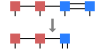
\includegraphics[scale=1.5]{figures/contraction_reseau}
  \end{center}
  \caption[Contraction de deux tenseurs]{
    La contraction de deux tenseurs d'un réseau.
    Cette contraction des tenseurs jaunes en bas à gauche du réseau
    en un nouveau tenseur de rang 3 correspond à l'équation~\eqref{eq:contraction_somme}.
  }
  \label{fig:contraction_reseau}
\end{figure}

À la section~\ref{sec:codes_polaires} et dans l'article associé à la thèse,
j'utiliserai plusieurs dizaines voir centaines de tenseurs pour 
représenter des distributions de probabilité.
Dans ce cas, 
la notation de sommation devient inutilisable 
en raison du nombre trop important de tenseurs et d'indices.
Pour contourner ce problème,
j'utiliserai une notation graphique pour les tenseurs.
C'est cette représentation graphique qui porte le nom de réseaux de tenseurs.

Un réseau de tenseur est défini par un graphe $G = (\tenseurs, \aretes)$\footnote{Je fais 
un rappel des notions de théorie des graphes à l'annexe~\ref{chap:theo_graphe}.} où $\tenseurs$ 
est un ensemble de tenseurs et $\aretes \subseteq (\tenseurs \times \tenseurs) \cup \tilde{\tenseurs}$ 
est un ensemble d'arêtes fermées, $\tenseurs \times \tenseurs$, reliant deux tenseurs 
et d'arêtes ouvertes, $\tilde \tenseurs = \qty{\qty{T} : T \in \tenseurs}$, comprenant un seul tenseur.
Une arête $a \in \aretes$ est connectée à un tenseur $T \in \tenseurs$ si $T \in a$.
Le rang d'un tenseur $T \in \tenseurs$ correspond au degré de $T$ dans $G$,
soit le nombre d'arêtes connectées à $T$.
Ainsi, chaque arête connectée à $T$ correspond à un indice de $T$.

Une arête fermée correspond à une paire d'indice à contracter entre deux tenseurs.
Suite à la contraction de ces indices, le réseau est modifié comme 
illustré à la figure~\ref{fig:contraction_reseau}.
Lors de la contraction d'une paire de tenseurs dans un réseau,
le nombre d'arêtes ouvertes du réseau est conservé.
La contraction d'un réseau de tenseurs est ainsi une séquence de contractions 
de paires de tenseurs jusqu'à ce qu'il ne reste qu'un seul tenseur avec des arêtes ouvertes.
Pour ce faire, 
il est important de considéré l'ordre des contractions pour minimiser la taille 
des tenseurs intermédiaires puisque cela peut avoir un impact considérable sur la mémoire
requise et le temps de calcul.
En effet,
il est possible que ces deux quantités augmentent exponentiellement avec le nombre 
de tenseurs et d'arêtes dans le réseau initial.
Trouver l'ordre de contraction optimal est un problème appartenant 
à la classe de complexité $\sharp P$\footnote{Je fais un rappel des notions de la 
théorie de la complexité à l'annexe~\ref{chap:complexite_calcul}. Dans ce cas, 
il est suffisant de comprendre qu'il s'agit d'un problème très difficile même 
en utilisant une grande quantité de ressources numériques.}~\cite{biamonte_tensor_2015}. 
Heureusement,
pour les codes polaires et les codes polaires convolutifs,
un ordre de contraction efficace se présente naturellement.


\section{Codes polaires}
\label{sec:codes_polaires}


C'est en 2009 que Arikan introduit les codes polaires~\cite{arikan_channel_2009}.
Le concept fondamentale derrière la construction des codes polaires est la polarisation
des canaux bruités.
Cette technique permet de convertir deux canaux bruités similaires en un canal moins bruité
et un canal plus bruité.
Ainsi,
un ensemble de canaux presque sans bruit et un ensemble presque inutilisable
sont obtenues en répétant itérativement cette approche à partir de plusieurs canaux similaires.
Ce qui est remarquable est que la fraction de canaux de faible bruit créés ainsi
tend vers la capacité des canaux initiaux.
En combinant cela au fait qu'il existe un algorithme efficace de décodage des codes polaires,
nous obtenons une famille de codes aux performances très prometteuse.
Dans le reste de cette section,
je vais d'abord introduire le procéssus de polarisation des canaux
avant d'introduire la construction des codes polaires
et de finalement présenter l'algorithme de décodage par réseaux de tenseurs. 

\subsection{Polarisation des canaux}

Je vais décrire un canal à partir de sa fonction de poids. 
Ainsi,
le canal binaire symétrique $\canal_p$ est représenté par la fonction de poids
\begin{equation}
  W_1(y|x) =
  \begin{cases}
    1 - p & \text{si } x = y,\\
    p & \text{si } x \neq y.\\
  \end{cases}
\end{equation}
Cette fonction représente la probabilité de recevoir $y$ si $x$ a été transmis.

Pour la construction des codes polaires,
des canaux plus généraux $W(\vb y | x)$,
où $\vb y \in \qty{0, 1}^m$ est un vecteur de $m$ bits,
sont considérés.
De plus, 
l'analyse se limite aux canaux composés de canaux binaires symétriques.
Dans ce cas, l'information mutuelle d'un canal décrit par $W(\vb y | x)$
est maximisée par une probabilité uniforme des valeurs de $x$.
La capacité est alors~\footnote{
  Sauf indication contraire, les logarithmes dans cette thèse sont calculés en base 2.
}
\begin{align}
  \capacite(W) 
  = I(X ; Y)
  &= \sum_{\vb y \in \qty{0, 1}^m}\sum_{x \in \qty{0, 1}} 
  \Pr(x, y) \log\qty(\frac{\Pr(x, y)}{\Pr(x) \Pr(y)})\notag\\
  &= \sum_{\vb y \in \qty{0, 1}^m}\sum_{x \in \qty{0, 1}} 
  \frac{1}{2}W(\vb y | x) \log\qty(\frac{2 W(\vb y | x)}{W(\vb y | 0) + W(\vb y | 1)})
  \label{eq:capacite_symetrique}
\end{align}
puisque $\Pr(x = 0) = \Pr(x = 1) = 1/2$.

La première étape de la polarisation est de combiner 
deux copies du canal binaire symétrique $W_1$ en un nouveau canal à 2 bits selon 
\begin{equation}
  W_2(\vb y_1^2 | \vb u_1^2) = W_1(y_2 | u_2) W_1(y_1 | u_1 + u_2),
\end{equation}
comme illustré à la figure~\ref{fig:polarisation}.
Dans cette section, je suis la littérature sur la correction d'erreurs
classique et j'utilise la notation $\vb x_i^j = (x_i, x_{i + 1}, \ldots x_j)$.
Le canal $W_2$ est obtenu en transformant l'entrée $(u_1, u_2)$ vers $(u_1 + u_2, u_2)$.
Cette transformation est l'analogue classique de la porte logique CNOT très utilisée 
en informatique quantique.

\begin{figure}[t]
  \begin{center}
    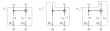
\includegraphics[scale=1.2]{figures/polarisation.pdf}
  \end{center}
  \caption[Polarisation des canaux]{
    Polarisation d'une paire de canaux.
    Le canal $W_2$ est obtenu en combinant deux canaux $W_1$ à l'aide de la porte CNOT.
    Le canal $W_2^{(1)}$ est obtenu en transmettant $u_1$ via $W_2$ lorsque $u_2$ est inconnu.
    Le canal $W_2^{(2)}$ est obtenu en transmettant $u_2$ via $W_2$ lorsque $u'_1$ est connu.
.  }
  \label{fig:polarisation}
\end{figure}

Comme de l'information sur le bit $u_2$ est transmise via les deux canaux initiaux et 
que seule de l'information partielle est transmise sur $u_1$ par le premier canal,
il est intuitif de croire que le bit $u_2$ sera mieux protégé des erreurs. 
C'est cette intuition que je vais maintenant formaliser.

Le canal $W_2$ est décomposé en un mauvais canal $W_2^{(1)}$ et un bon canal $W_2^{(2)}$.
Pour ce faire,
les bits $u_1$ et $u_2$ sont transmis de façon successive.
D'abord, 
le bit $u_1$ est transmis en ignorant la valeur de $u_2$. 
Le mauvais canal,
\begin{equation}
  W_2^{(1)}(\vb y_1^2 | u_1) 
  = \sum_{u_2 \in \qty{0, 1}} W_2(\vb y_1^2 | u_1^2) \Pr(u_2)
  = \frac{1}{2}\sum_{u_2 \in \qty{0, 1}} W_1(y_2 | u_2) W_1(y_1 | u_1 + u_2),
\end{equation}
est obtenu en supposant qu'il est équiprobable que $u_2 = 0$ et $u_2 = 1$.

Pour retrouver la valeur de $u_1$ transmise par ce canal, 
la valeur de $u_2$ est estimée selon $W_1(y_2 | u_2)$. 
La probabilité de succès est de $1 - p$. 
Ensuite, 
la valeur de $u_1$ est estimée selon $W(y_1 | u_1 + u_2)$.
En supposant la bonne valeur de $u_2$, 
la probabilité de succès de cette étape est également de $1 - p$.
Ainsi, la probabilité totale de succès est de $(1 - p)^2$,
ce qui est inférieure à la probabilité de succès $1 - p$ de $W_1$.

\begin{figure}
  \begin{center}
    \includegraphics{figures/capacite_polarisation.pdf}
  \end{center}
  \caption[Capacité des canaux polarisés]{Comparaison de la capacité des canaux polarisés.}
  \label{fig:capacite_polarisation}
\end{figure}

Le bon canal est construit en supposant que la valeur de $u_1$ est connue,
soit parce qu'elle est fixée initialement ou qu'elle a été retrouvée avec succès
après l'utilisation du mauvais canal.
La fonction de poids du bon canal est alors
\begin{equation}
  W_2^{(2)}(\vb y_1^2, u'_1 | u_2) 
  = W_1(y_2 | u_2) W_1(y_1 | u'_1 + u_2),
\end{equation}
où la valeur $u'_1$ est connue. 
Dans le cas où $u_1 = 0$, 
utiliser ce canal est équivalent à envoyer deux copies de $u_2$. 
Ainsi, 
s'il y a une seule erreur, alors $y_1 \neq y_2$ et il est possible de détecter l'erreur.
Une erreur doit donc affecter chacun des bits pour que celle-ci ne soit pas détecter.
Cela a une probabilité $p^2$ ce qui est inférieure à la probabilité d'échec $p$ du canal $W_1$.
Une logique similaire s'applique lorsque $u_1 = 1$.

La capacité des différents canaux est calculée à partir 
de l'équation~\eqref{eq:capacite_symetrique}
et est illustrée à la figure~\ref{fig:capacite_polarisation}.
À l'exception des cas où la correction d'erreurs est inutile,
soit lorsque $p = 0$, $p =0.5$ ou $p = 1$,
il est clair, selon la figure, qu'il y a un avantage à utiliser le bon canal $W_2^{(2)}$.
Par exemple, pour $p = 0.2$, la capacité de celui-ci est près du double 
de la capacité initiale et plus de 4 fois supérieure à la capacitié du mauvais canal $W_2^{(1)}$.

\subsection{Construction des codes polaires}

L'astuce derrière la construction des codes polaires est de repéter itérativement le 
processus de polarisation des canaux.
En effet, 
en répérant cet opération sur deux bons canaux obtenus par polarisation,
nous obtenons un nouveau canal encore plus performant et un canal de qualité moyenne.
De même,
en polarisant deux mauvais canaux, nous obtenons un canal de qualité moyenne et 
un canal médiocre.
En répétant ce procédé un très grand nombre de fois,
Arikan a montré~\cite{arikan_channel_2009} 
que la fraction des canaux atteignant une capacité de 1
tend vers $1 - H_2(p)$, soit la capacité des canaux initiaux.
L'idée est alors d'utiliser ces canaux pour transmettre l'information
et fixer la valeur des autres bits à 0.

\begin{figure}
  \begin{center}
    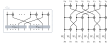
\includegraphics[scale=1.3]{figures/circuit_code_polaire.pdf}
  \end{center}
  \caption[Circuit des codes polaires]{
    Circuit d'encodage pour les codes polaires.
    À gauche, la relation de récurrence pour ajouter un niveau de polarisation.
    À droite, la transmission de 8 bits encodés à l'aide de trois niveaux de polarisation.
  }
  \label{fig:circuit_code_polaire}
\end{figure}

De façon similaire à la polarisation d'une paire de canaux,
la polarisation de $n = 2^m$ canaux s'effectue en combinant
d'abord les $n$ canaux $W_1$ en un seul canal,
\begin{equation}
  W_n(\vb y_1^n | \vb u_1^n) = \prod_{i=0}^n W_1(y_i | x_i),
\end{equation}
où $\vb x_1^n = G_n \cdot \vb u_1^n$.
Le circuit d'encodage $G_n$ est obtenu de manière récursive à partir de la relation illustrée
à la figure~\ref{fig:circuit_code_polaire} et en considérant 
\begin{equation}
  G_2 = 
  \begin{pmatrix}
    1 & 1 \\
    1 & 0
  \end{pmatrix}.
\end{equation}
Pour ajouter un niveau de polarisation,
le bit d'indice $1 \leq i \leq 2^{m-1}$ et le bit 
d'indice $i + 2^{m-1}$ sont connectés à l'aide de la
transformation $G_2$ correspondant à la porte CNOT.

Par la suite,
le canal $W_N$ est décomposé en une série de canaux,
\begin{equation}
  W_n^{(i)}(\vb y_1^n, \vb u_1^{i - 1} | u_i) 
  = \frac{1}{2^{n - i}}
  \sum_{u_{i+1}^n \in \qty{0, 1}^{n - i}} W_n(\vb y_1^n | \vb u_1^n),
  \label{eq:canal_polarise}
\end{equation}
permettant la transmission d'un bit.
Ainsi, 
le bit $u_i$ est transmis en connaissant la valeur des bits précédents et en 
ignorant la valeur des bits suivants de probabilité uniforme.
Il reste alors à trouver l'ensemble des canaux ayant les plus grandes capacités
et de fixer la valeur des autres bits à 0.
Cela engendre un protocole de communication permettant d'envoyer des messages de
$k \to n(1 - H_2(p))$ bits encodés à l'aide de $n = 2^m$ bits, ce qui est optimal pour le 
canal binaire symétrique.

Il est évident que le bit $u_n$ est le mieux protégé puisqu'il se retrouve
toujours du bon côté de la polarisation. 
De même, 
le bit $u_1$ est le plus bruyant, car il est toujours du mauvais côté.
Cependant, 
il est plus difficile d'ordonner les bits centraux qui se retrouve parfois du bon côté
et parfois du mauvais.
Il est tentant d'essayer de calculer la capacité de chacun des canaux et des les ordonner
ainsi.
Cependant, ce calcul implique la somme de $2^n$ termes pour chacun des canaux. 
Il est alors impossible de faire ce calcul en un temps raisonnable.
Il existe quelques façons de contourner ce problème.
D'abord Arikan~\cite{arikan_channel_2009} propose d'utiliser le paramètre de Bhattacharyya,
\begin{equation}
  Z(W) = \sum_{\vb y} \sqrt{W(\vb y|0)W(\vb y|1)},
\end{equation}
qui est relié à la capacité par
\begin{equation}
  \log\qty( \frac{2}{1 + Z(W)} )
  \leq  
  \capacite(W) 
  \leq 
  \sqrt{1 - Z(W)^2} .
\end{equation}
L'avantage du paramètre de Bhattacharyya est qu'il existe un algorithme récursif pour
calculer sa valeur pour l'ensemble des canaux en temps polynomial.

Dans l'article associé à cette thèse, 
je présente une autre approche plus simple, 
mais un peu moins précise, 
pour choisir les canaux.

\subsection{Décodage par réseaux de tenseurs}

Dans cette section,
je présente un décodeur par réseaux de tenseurs pour les codes polaires 
inspiré du décodeur à annulation successive introduit par Arikan~\cite{arikan_channel_2009}.
Ce décodeur par réseaux de tenseurs à d'abord été présenté par Ferris 
et Poulin~\cite{ferris_branching_2014} et c'est ce qui a permi 
la construction des codes polaires convolutifs étudiés dans l'article associé à cette thèse.

Pour la suite, 
je définie un code polaire en fonction du nombre de niveaux de polarisation $m$
et d'un ensemble de bits $\mathcal F$ dont la valeur est fixée à 0.
Chacun des $n = 2^m$ bits d'un tel code sont décodés de manière successive.
C'est-à-dire, 
après avoir reçu le message $\vb y$,
pour trouver la séquence de bit $\vb u$ la plus probable,
le bit $u_1$ est décodé, suivit du bit $u_2$ et ainsi de suite jusqu'à décoder le bit $u_n$.
Dans le cas où $i \in \mathcal F$, 
il est inutile de décoder le bit $u_i$ et il suffit de lui assigner la valeur fixe $0$.
Dans le cas contraire,
il est possible de construire un réseau de tenseurs contractable en temps $\bigO(n)$
pour obtenir un vecteur dont les éléments sont $W_n^{(i)}(\vb y_1^n, \vb u_1^{i-1} | 0)$
et $W_n^{(i)}(\vb y_1^n, \vb u_1^{i-1} | 1)$.
Il suffit alors de choisir 
\begin{equation}
  u_i = \max_{u_i' \in \qty{0,1}} W_n^{(i)}(\vb y_1^n, \vb u_1^{i-1} | u_i').
\end{equation}
Dans le reste de cette section,
je vais décrire comment construire et contracter le réseau de tenseur
pour décoder chacun de ces bits.

D'abord, 
un réseau de tenseur général est construit
pour l'entièreté du décodage.
Celui-ci se simplifie en un réseau de tenseurs en forme d'arbre
lors du décodage de chacun des bits,
Le réseau général est composé de quatre tenseurs de bases,
soit les deux vecteurs
\begin{align}
  &\vcenter{\hbox{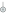
\includegraphics{figures/tenseur_0.pdf}}}
  =\begin{pmatrix}1\\0\end{pmatrix},
  &&\vcenter{\hbox{
\includegraphics{figures/tenseur_1.pdf}}}
  =\begin{pmatrix}0\\1\end{pmatrix},
  \label{eq:tenseurs_01}
\end{align}
et les deux tenseurs de rang supérieur
\begin{align}
  &\vcenter{\hbox{
\includegraphics{figures/tenseur_w.pdf}}}
  =
  \begin{pmatrix}1 - p & p \\ p & 1 - p\end{pmatrix}, 
  &&\vcenter{\hbox{
\includegraphics{figures/tenseur_cnot.pdf}}}
  =
  \begin{cases}
    1 & \text{si } i = j, k \neq l, \\
    0 & \text{sinon}.
  \end{cases}
  \label{eq:tenseurs_cp}
\end{align}
Les éléments de ses vecteurs sont tous des nombres réels et non des éléments de $\bit$.

\begin{figure}
  \begin{center}
    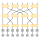
\includegraphics[scale=1.3]{figures/reseau_tenseurs_codes_polaires.pdf}
  \end{center}
  \caption[Exemple d'un réseau de tenseur pour décoder un code polaire]{
    Réseau de tenseurs pour le décodage d'un code polaire à 3 niveaux de polarisation.
  }
  \label{fig:reseau_tenseurs_codes_polaires}
\end{figure}

Pour $y_i \in \qty{0, 1}$,
la fonction de poids $W_1$ s'obtient par la contraction
\begin{equation}
  \vcenter{\hbox{
\includegraphics{figures/contraction_y_w.pdf}}}
  =
  \begin{pmatrix}
    W_1(y_i | 0) \\
    W_1(y_i | 1)
  \end{pmatrix}
  =
  \begin{cases}
    \begin{pmatrix}1 - p\\p\end{pmatrix} & \text{si } y_i = 0, \\[0.7cm]
    \begin{pmatrix}p\\1-p\end{pmatrix} & \text{si } y_i = 1.
  \end{cases}
\end{equation}
La réseau complet est alors obtenu en connectant les contractions $W \cdot y_i$
au circuit d'encodage du code où les portes CNOT sont remplacées par le tenseur 
de rang 4 de l'équation~\eqref{eq:tenseurs_cp} comme illustré à la 
figure~\ref{fig:reseau_tenseurs_codes_polaires}.
Le réseau résultant correspond alors à la fonction de poids $W_n(\vb y_1^n | \vb u_1^n)$
où les valeurs de $\vb u_1^n$ correspondent aux indices ouverts du réseau.

\begin{figure}
  \begin{center}
    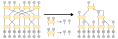
\includegraphics[scale=1.3]{figures/simplification_codes_polaires.pdf}
  \end{center}
  \caption[Exemple de simplification de la contraction d'un code polaire]{
    Exemple de simplification de la contraction pour un code polaire à 3 niveaux de polarisation.
    Les transformations utilisées sont données à l'équation~\eqref{eq:simplification_codes_polaires}.
  }
  \label{fig:simplification_codes_polaires}
\end{figure}

Pour obtenir le canal polarisé de l'équation~\ref{eq:canal_polarise},
un vecteur parmi les deux choix présentés à l'équation~\ref{eq:tenseurs_01}
est connecté à chacun des indices ouverts correspondant aux bits $\vb u_1^{i-1}$
selon les valeurs (0 ou 1) précédemment décodées.
Le vecteur 
\begin{equation}
  \vcenter{\hbox{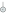
\includegraphics{figures/tenseur_e.pdf}}}
  =\begin{pmatrix}1\\1\end{pmatrix}
\end{equation}
est connecté aux indices ouverts des bits $\vb u_{i+1}^{n}$ pour sommer
sur les valeurs encore inconnues.
Ce vecteur ne prend pas en compte la normalisation,
mais cela ne fait que multiplier les éléments du réseau de tenseur
contracté par une constante globale n'ayant pas d'impact sur la calcul de
la valeur maximum.

Il est possible de simplifier ce réseau de tenseur à l'aide des relations
\begin{align}
  &\figeq{contraction_cnot_e_e} = \figeq{tenseurs_e_e},
  &&\figeq{contraction_cnot_u_v} = \figeq{tenseurs_u_w},
  \label{eq:simplification_codes_polaires}
\end{align}
où $u, v \in \qty{0, 1}$ et $w = u + v$ tel qu'illustré à la 
figure~\ref{fig:simplification_codes_polaires}.
Le résultat de ces simplifications sera toujours un réseau de tenseurs
en forme d'arbre~\cite{ferris_branching_2014} puisqu'au niveau de polarisation
$l$, seulement $2^{m - l}$ ne peuvent pas être simplifiés.

L'avantage des réseaux de tenseurs en forme d'arbre est qu'il est possible de 
les contracter efficacement~\cite{arad_quantum_2010}.
Dans le cas présent,
il suffit de contracter le réseau de tenseur en partant du premier niveau de polarisation
vers le dernier comme illustré à la figure~\ref{fig:contraction_codes_polaires}.
Le coût de cette contraction est de $\bigO(2^m)$.
Ainsi,
le coût total du décodage pour un code de $n = 2^m$ est au plus $\bigO(n^2)$ puisque 
$n$ bits doivent être décodés.
Cependant,
il est possible de faire mieux en observant que les réseaux simplifiés partagent des sous-réseaux
communs.
Par exemple,
lors du décodage des bits $u_1$ et $u_2$, 
seule la contraction au dernier niveau de polarisation est différente puisque les 
vecteurs associés aux bits $\vb u_3^n$ restent inchangés et engendrent les même simplifications.
En réutilisant les calculs déjà effectués,
le coût du décodage devient $\bigO(n\log(n))$~\cite{ferris_branching_2014, arikan_channel_2009}.

\begin{figure}
  \begin{center}
    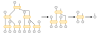
\includegraphics[scale=1.3]{figures/contraction_codes_polaires.pdf}
  \end{center}
  \caption[Exemple de contraction d'un code polaire]{
    Exemple de contraction d'un réseau de tenseurs en forme d'arbre 
    pour un code polaire à 3 niveaux de polarisation.
    À chaque étape, les tenseurs de rang 4 du niveau inférieur sont contractés
    avec trois vecteurs.
    À la première étape, 
    les tenseurs correspondant aux paires $W$ et $y_i$ sont déjà contractée.
  }
  \label{fig:contraction_codes_polaires}
\end{figure}

Le coût du décodeur par réseaux de tenseurs est similaire au décodeur par annulation successive introduit
en même temps que les codes polaires.
Ces décodeurs combinés au fait qu'il est possible de transmettre de l'information à 
un rendement $1 - H_2(p)$ font des codes polaires les premiers codes correcteurs permettant 
d'atteindre la capacité d'un canal tout en étant efficacement décodable.

\section{Comparaison de la profondeur et de la largeur des codes polaires convolutifs}

Les codes polaires convolutifs sont une généralisation des codes polaires.
Ferris et Poulin~\cite{ferris_branching_2014} ont introduit ces codes
en se basant sur la structure en arbre du réseau de tenseurs pour 
chacune des étapes du décodage.
En effet, 
toutes les modifications aux circuits des codes polaires qui permettent
de conserver cette structure engendrent une famille de codes décodable
avec un coût $\bigO(n \log(n))$.
La première modification proposée est d'ajouter 
une couche de portes CNOT décalée de 1 bit à chaque niveau de polarisation.
La figure 1a de l'article joint à cette thèse illustre bien cette construction.

Par la suite,
dans le cadre de cette thèse,
j'ai généralisé cette construction de deux façons.
D'abord,
j'ai ajouté des couches de portes à chaque niveau de polarisation.
La profondeur (\textit{depth}) d'un code polaire convolutif est
alors le nombre de couches par niveau.
Ensuite, j'ai remplacé la porte CNOT qui
permet de polariser deux canaux par des portes qui permettent de polariser plusieurs 
canaux simultanément.
La largeur (\textit{breadth}) d'un code polaire convolutif est le nombre de
canaux polarisés par porte.
Pour une largeur $b$, 
la transformation
\begin{equation}
  (u_1, u_2, \ldots, u_{b-1}, u_b) 
  \to 
  (u_1 + u_2, u_2 + u_3, \ldots, u_{b-1} + u_b, u_b) 
\end{equation}
est utilisée.

La figure 1 de l'article présente plusieurs exemples de ces deux généralisations.
On y voit également qu'un code polaire régulier est équivalent à un code polaire convolutif
de profondeur 1 et de largeur 2.

Dans l'article,
je compare l'impact de la profondeur et de largeur sur les performances des codes.
De plus, 
bien que la coût du décodage de chacun de ces codes soit de $\bigO(n \log(n))$,
augmenter la profondeur ou la largeur augmente la coût d'un facteur multiplicatif constant.
Ainsi,
considérant les performances impressionnantes des codes polaires,
il est important de comprendre comment cette augmentation du coût de décodage 
se compare à l'augmentation des performances
afin d'estimer s'il est rentable de généraliser ces codes.

Je réponds à cette question à montrant d'abord que la performance des codes 
augmentent avec la profondeur et diminue avec la largeur.
Suite à cela, une étude du coût de décodage permet de conclure qu'il est optimal
d'utiliser des codes de profondeur et largeur 2 puisque le gain de performance 
pour des profondeurs plus élévées est moins appréciable.

\subsection{Contribution}

Pour cet article,
j'ai implémenté, 
assisté par Benjamin Bourassa, 
un logiciel qui permet de simuler le décodage des codes polaires convolutifs.
Par la suite,
j'ai effectué les simulations Monte Carlo qui ont permis d'évaluer la performance
des divers codes correcteurs et j'ai fait l'analyse de ces résultats.
J'ai également écrit l'article avec l'aide du professeur David Poulin
qui a supervisé l'ensemble du projet.

\subsection{Article}

Cet article ayant pour titre original \textit{Depth versus Breadth in Convolutional Polar Codes}
a été publié en 2018 dans la cadre de la conférence \textit{IEEE Information Theory Workshop}.

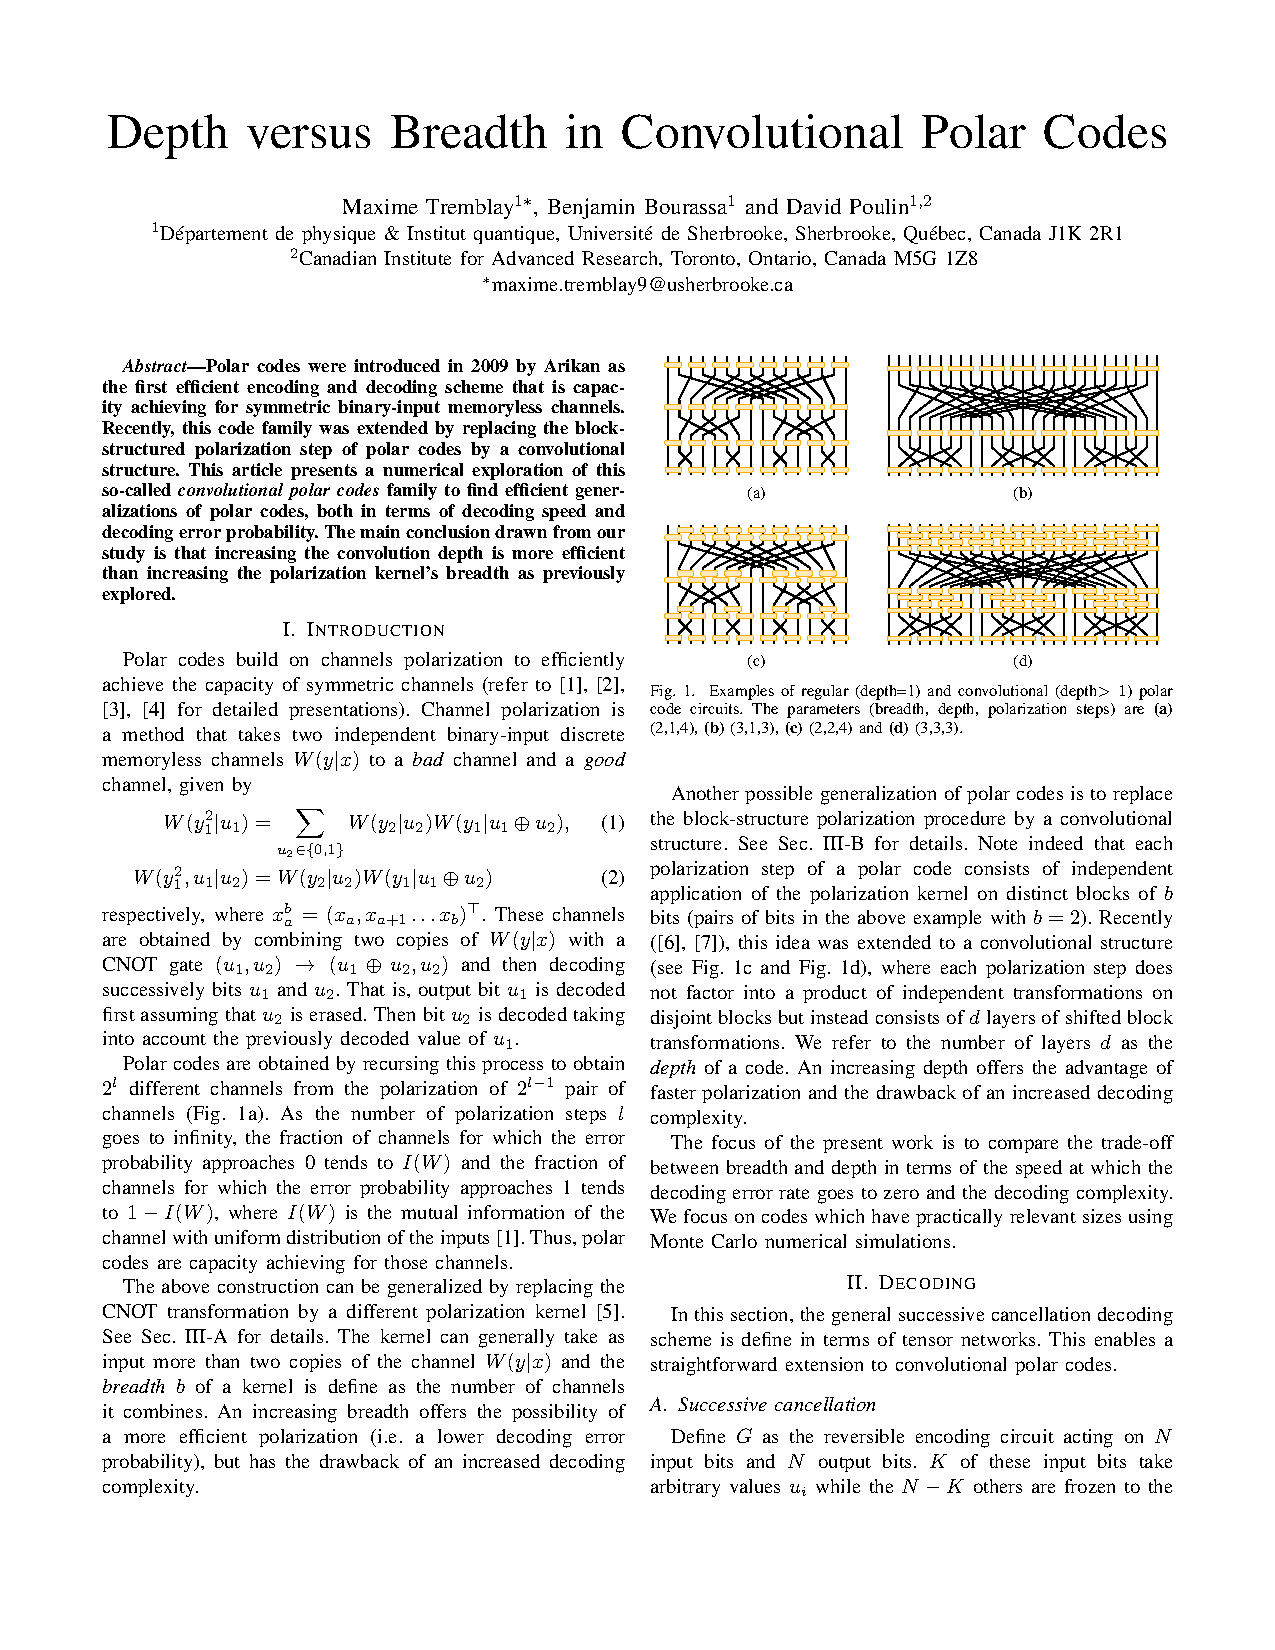
\includepdf[pages=-]{articles/conv_polar_codes.pdf}
